\chapter{Results and Discussion}
\section{Precision, Recall and F1 Scores Comparison}
In 2 out of 3 algorithms, our term-recency modification improved the performance notably. When measured by p@10, tTF-IDF outperformed TF-IDF by an average 47\% and tUSE outperformed USE in 2 of the 3 datasets by average 14.3\% but performed 50\% worse in the third dataset (shown in Figure \ref{fig:tf-idf-precision-comparison} and \ref{fig:use-precision-Comparison}). The time normalized BM25 version, however, performed 32\% worse than BM25 (shown in Figure \ref{fig:bm25-precision-comparison}). 


In the general case of Information retrieval evaluation, Recall and F1 measures give different results than precision metrics, if the given number of relevant results are not fixed. In our datasets, only TREC news has a varied number of relevant results given as ground truth. In other cases, if the number of given relevant results are constant, then all three values, that is precision, recall and F1 scores remain the same. 
In case of TREC news dataset, for calculating the recall and F1 scores, we fetch the top 100 results for the given query sets. For uniformity in the metric calculation, we compute the precision scores as well. The result metrics are shown in \textit{Figure \ref{fig:recall-f1-metrics}}. Recall and F1 scores as well show a significant improvement of time normalized models over the standard ones. Evaluating in terms of recall, we see a 93\% improvement in the tTF-IDF model over TF-IDF and a 28\% improvement in tUSE model over the USE model. While tBM25 performed 27\% worse than the standard BM25 model.

\begin{figure}
    \centering
    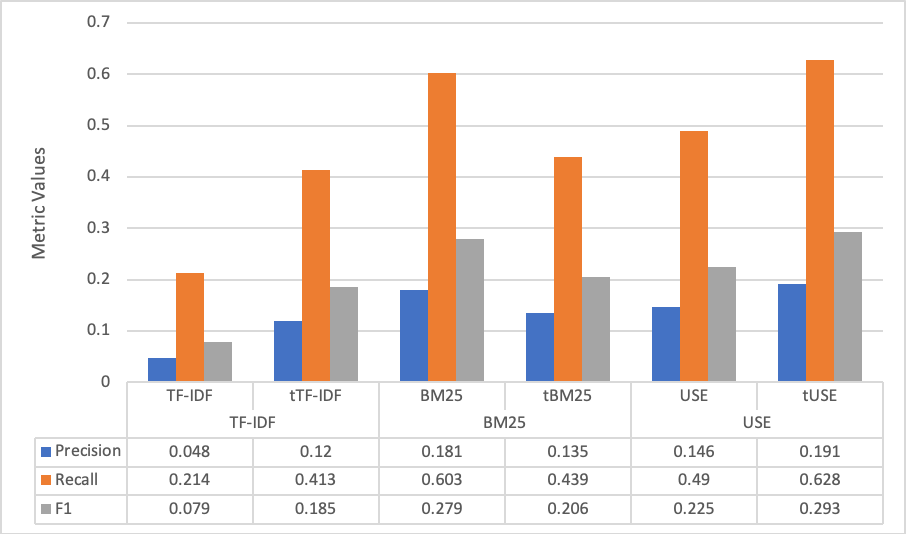
\includegraphics[width=\textwidth]{recall-f1scores.png}
    \caption{Precision, Recall, F1@100 scores for TREC News }
    \label{fig:recall-f1-metrics}
\end{figure}

\subsection{tTF-IDF vs TF-IDF}
On comparing in terms of precision and NDCG scores, tTF-IDF model outperformed TF-IDF model in all three datasets. Digging deep into the results, for TREC news dataset, we see a massive improvement of 115\% in the precision score. While for CiteULike tTF-IDF outperformed TF-IDF by 11\% and for WebAP dataset, tTF-IDF outperformed by 15\% (shown in Figure \ref{fig:tf-idf-precision-comparison}).
Based on the study of corpus and results retrieved for each dataset, the following inferences can be derived:
\begin{itemize}
    \item presence of temporal context in a news corpus is high compared to other text corpora. The reason for such an assumption is that news highlights events of a different era, having a higher chance of showing time relation compared to any other text
    \item Size of the corpora is different and so the variation in the term age is another factor. Since the term age is also dependent on the document frequency, so the size of corpus also affects the term age indirectly.
    \item Term age might not be adding much relevance to CiteULike and WebAP dataset, but performs significantly well to introduce the term age for improving results. And the results could be improved by testing out with different normalization factors for term age as well as tTF-IDF.
\end{itemize}
\begin{figure} [h!]
    \centering
    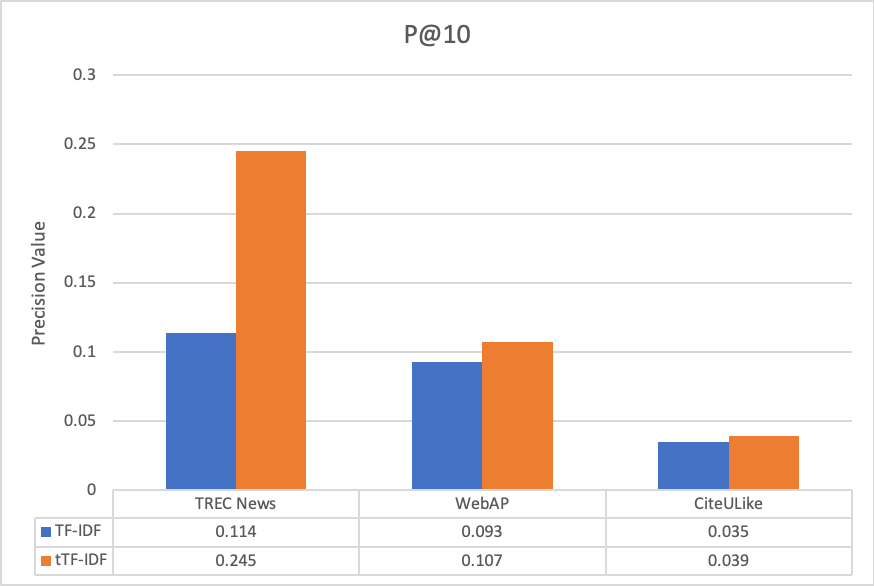
\includegraphics[width=120mm,scale=0.5]{p-10-tf-idf.png}
    \caption{TF-IDF vs tTF-IDF Precision Comparison}
    \label{fig:tf-idf-precision-comparison}
\end{figure}
\subsection{tBM25 vs BM25}
Time normalized BM25 model did not perform well for any of the datasets. tBM25 model performed 9.4\% worse for TREC news dataset, 44\% worse for CiteULike dataset, and 42.8\% worse for the Web AP dataset (shown in \ref{fig:bm25-precision-comparison}).
On closer analysis of the BM25 model, we see 27 out of 50 queries in TREC news task, gave better or almost similar results in case of time normalized BM25 model when compared to the classic approach. Assuming that the news text has a temporal context in them, these results are also promising and need to be worked upon for improvised results in future work.
Based on the results retrieved and study, the following inferences can be derived for tBM25 model:
\begin{itemize}
    \item BM25 and tBM25 model performs better than the classic TF-IDF and tTF-IDF model for all cases. 
    \item current term age formulation is not improvising the BM25 search algorithm. Different term age formulation or normalization factors need to be tested to verify the significance of term age in the BM25 algorithm.
    \item The reason for the worse performance of tBM25 model can also be because of the additional metric field length and average field length used in the BM25 formula. It might be possible that the current term age formulation does not fit in well with the field length metrics.
    \item Tuning of other constant parameters in BM25 formula, that is k1 and b can also be tried to improvise upon the tBM25 model.
\end{itemize}
\begin{figure} [h!]
    \centering
    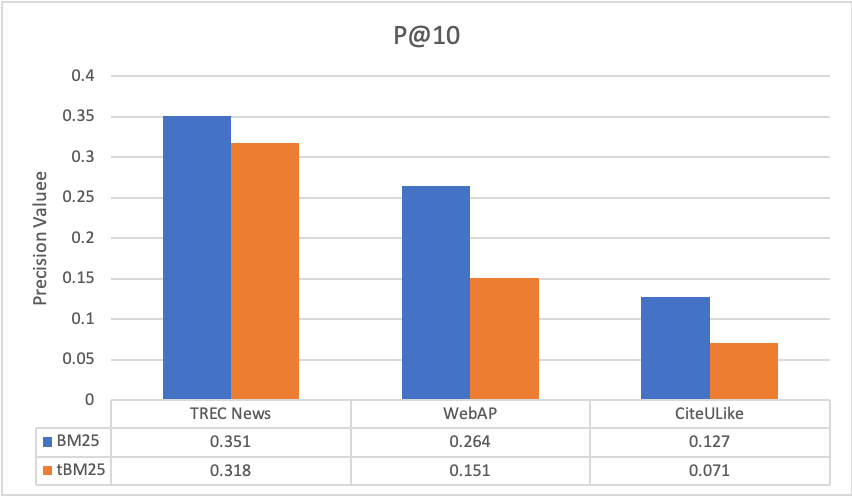
\includegraphics[width=120mm,scale=0.5]{p-10-bm25.png}
    \caption{BM25 vs tBM25 Precision Comparison}
    \label{fig:bm25-precision-comparison}
\end{figure}
\subsection{tUSE vs USE}
Time normalized Universal Sentence Encoder(tUSE) model outperformed the USE model in 2 of the 3 datasets. For TREC News dataset we observed 18\% improvement in tUSE model over standard USE. And in CiteULike, we get a 10.67\% improvement in the time normalized version. While it performed 50\% worse for the Web AP dataset. 

Analyzing the tUSE model in WebAP dataset, we see it does not perform well against the USE model. One of the possible reasons for this might be the size of the corpus used, that is, TREC news corpus has approximately 600k documents while Web AP dataset has just 6k documents, which is 100 times less than the former dataset. However, this is an inference based on the results retrieved and has not been verified. There might be other possible reasons, such as the size of documents, size of queries used, number of proper nouns in the queries, etc. Or probably term age might not be a relevant metric for this dataset. These possible reasons still need to be analyzed before affirming out a conclusion on these contrasting results.

Based on the study of corpus and results retrieved for each dataset, the following inferences can be derived:
\begin{itemize}
    \item out of TF-IDF, BM25, and USE, USE model performs best for fetching results for queries in the English language. And apparently, tUSE model performs better for 2 of the three datasets.
    \item currently implemented time normalization does not work well with the Web AP dataset in case of USE based relevance scoring.
    \item For background linking task in TREC news dataset, USE gave a p@10 value 0.52 while tUSE gave p@10 value of 0.614, which is far better compared to TF-IDF(0.114) and tTF-IDF(0.245). From this observation, it is evident that the semantics-based search is more promising than keyword-based search for such tasks.
\end{itemize}
\begin{figure} [h!]
    \centering
    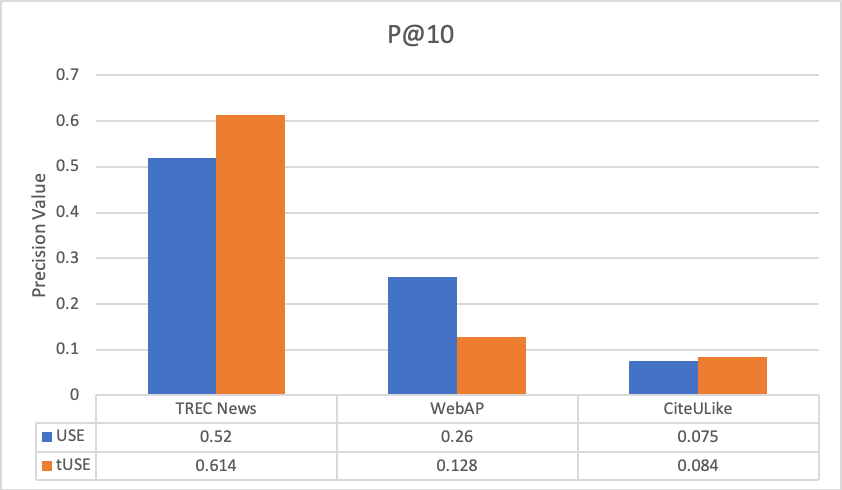
\includegraphics[width=120mm,scale=0.5]{p-10-USE.png}
    \caption{USE and tUSE Precision Comparison}
    \label{fig:use-precision-Comparison}
\end{figure}
\section{NDCG Score Analysis}
NDCG is used to evaluate the ranking measure of the results retrieved. we have used the top 10 results to validate the NDCG scores. And NDCG@10 leads to similar results as seen for precision@10, illustrated in section 7.1. We have calculated the NDCG scores only for TREC News and WebAP datasets, for CiteULike dataset, NDCG cannot be calculated, since this is based on the references used in the research paper and there is no ranking specified for the citations. 
For TREC news, we see tTF-IDF outperformed TF-IDF by 59\% and tUSE outperformed USE model by 10.76\%. While for tBM25 performed 18.3\% worse than the BM25 model. These comparison results are shown in figure \ref{fig:ndcg-scores}. 
Based on these NDCG scores and the p@10 metrics, it is evident that time normalized models are promising and have a wide scope of applications in information retrieval and recommendation systems.


\begin{figure}
    \centering
    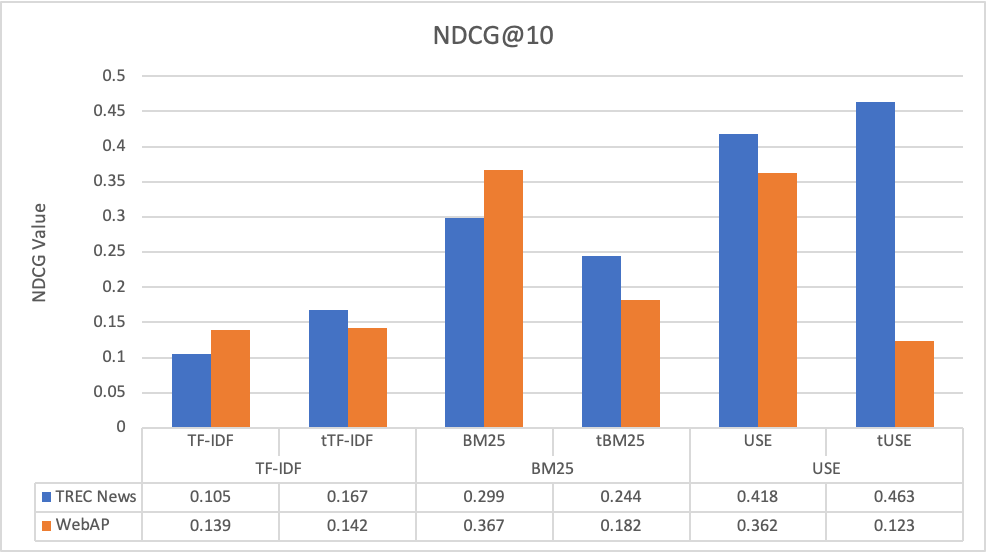
\includegraphics[width=\textwidth]{ndcg-comparison.png}
    \caption{NDCG@10 Score Comparison}
    \label{fig:ndcg-scores}
\end{figure}


\section{Term Age Distribution Analysis}
Looking at the distribution of words and their origin years, we observe a vast range of origin ranging from the year 1100 to the year 2015, illustrated in Figure \ref{fig:origin-year-distribution}. Most of the terms used are in the year range of 1800-1900, followed by year range 1500-1600. For TREC news dataset, we observed the document frequency ranges from 2 to 550k. Combining both of them, we get the term age ranging from 0 to 9.71, with a mean of 0.9308 and median of 0.1568. 
Similarly for other datasets, we observed a similar pattern of origin year but a change in the document frequencies. And consequently, variation in the term age is observed in the CiteUlike and Web AP dataset.Distribution Statistics for term age is shown in Table \ref{table:7.1}.

\begin{table}[h!]
\centering
\begin{tabular}{ |c|c|c|c|c|c|c| }
 \hline
 \textbf{Min.}	& \textbf{Mean} & \textbf{3rd quartile} & \textbf{Max.} & \textbf{Median} & \textbf{Std. dev.} & \textbf{Variance}\\
 \hline
 0 & 0.9308 & 1.5198 & 9.7120 & 0.1568 & 1.3363 & 1.7856 \\
\hline
\end{tabular}
\caption{Term Age Distribution}
\label{table:7.1}
\end{table}


\begin{figure}
    \centering
    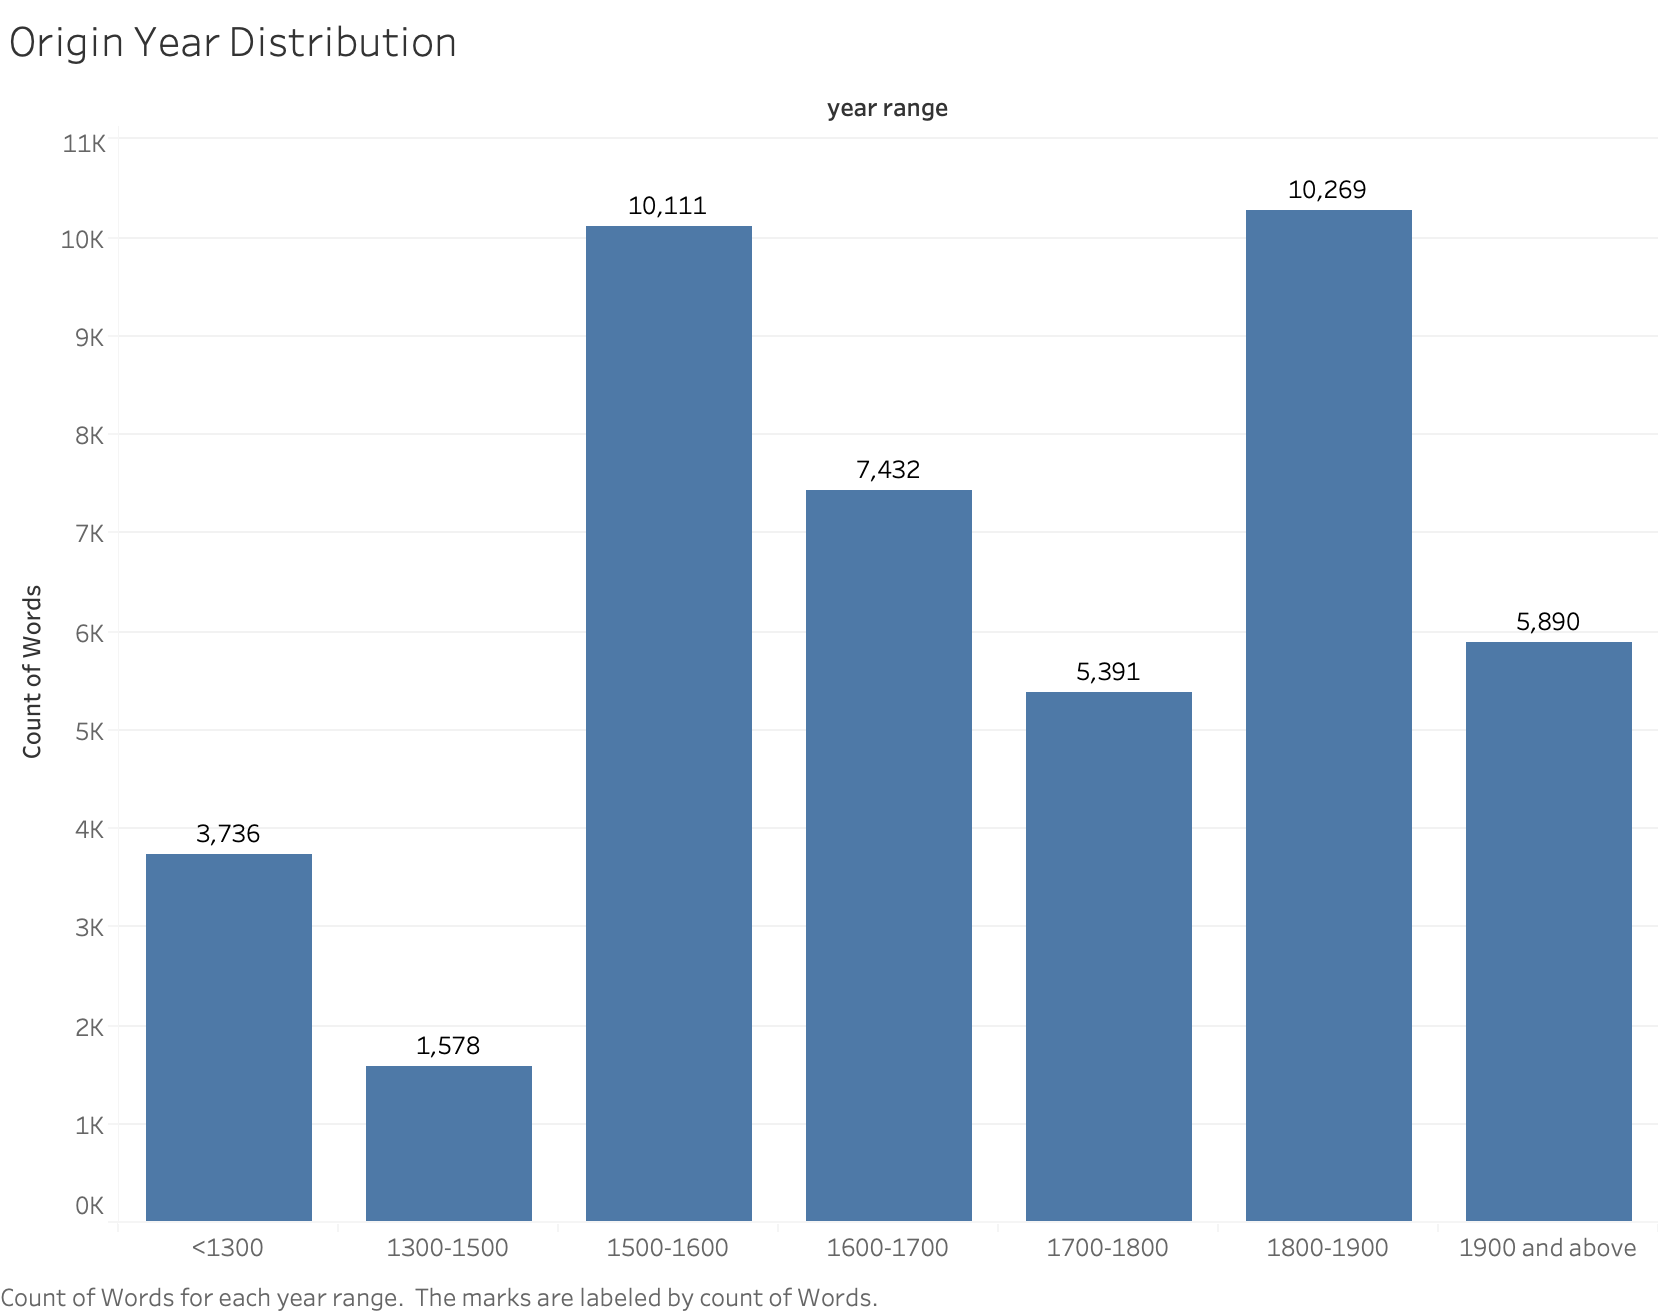
\includegraphics[width=100mm,scale=0.7]{origin year distribution.png}
    \caption{Origin Year Distribution in years}
    \label{fig:origin-year-distribution}
\end{figure}

\begin{figure}[h!]
    \centering
    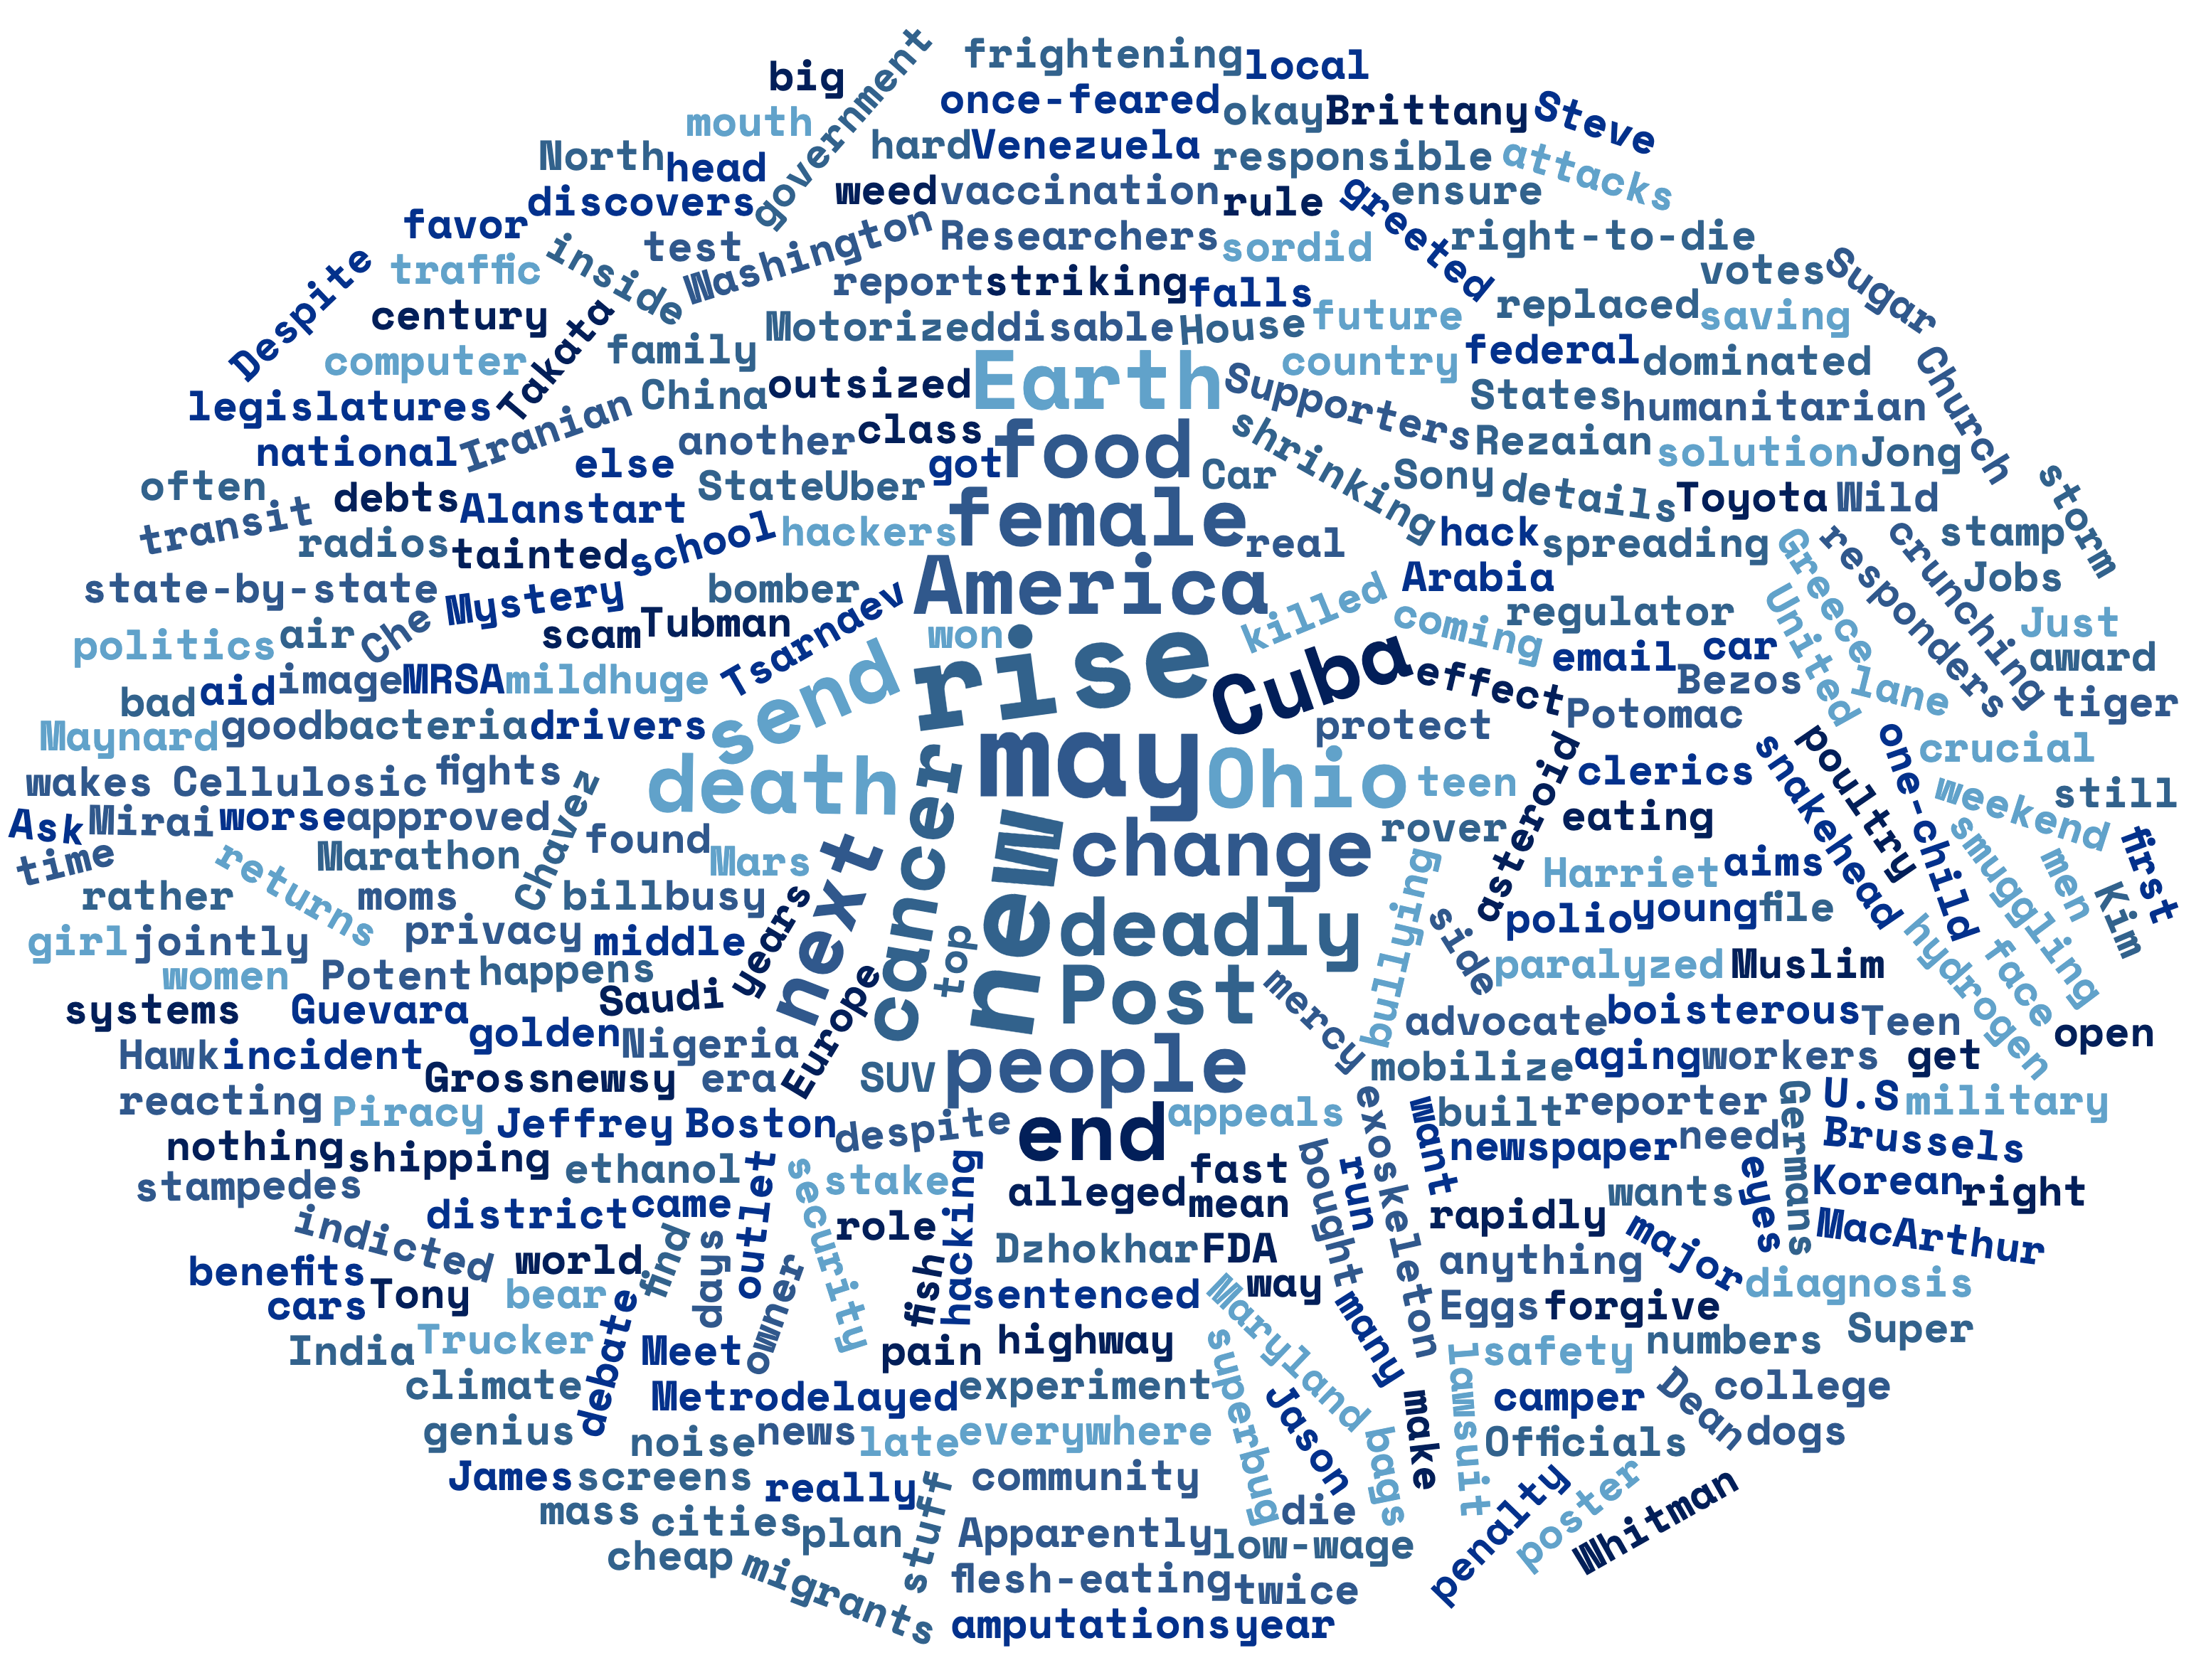
\includegraphics[width=140mm,scale=0.5]{searched-wordcloud.png}
    \caption{Searched words cloud in TREC News Dataset}
    \label{fig:search-word-cloud}
\end{figure}

Another interesting statistic to look at is the searched words and their frequency of search. We did analyse the searched terms pattern in for the TREC news background linking task and a word cloud for the searched words is shown in Figure \ref{fig:search-word-cloud}. In the word cloud, the size of the term shows the frequency of the term used. Most frequent terms in the search queries are, 'America', 'Cuba', 'Ohio', 'Change', 'deadly', 'rise', 'new', 'death', cancer', 'female', 'food', 'Earth' and some more terms that are shown in Figure \ref{fig:search-word-cloud}. 